\documentclass[11pt]{article}
\usepackage{geometry}
\usepackage{amsmath,amssymb,amsthm,mathrsfs, bm}
\usepackage{mathtools}
\usepackage{latexsym,amscd,amsbsy,dsfont,amsfonts}
\usepackage{graphicx}
\usepackage{xcolor}
\usepackage[pdftex,colorlinks=true]{hyperref}
\usepackage{caption}
\usepackage{physics}
\usepackage{tensor}
\usepackage{tikz}
\usetikzlibrary{bayesnet}
\usetikzlibrary{fit}
\usepackage[most]{tcolorbox}
\tcbuselibrary{theorems}
\usepackage{empheq}
\usepackage{enumitem}

% Number equation by section
\numberwithin{equation}{section}

% Page Layout
\geometry{
 a4paper,
 left=20mm,
 right=20mm,
 top=20mm,
}

%%%%%%%% Custom Commands %%%%%%%%%%%
% Shorthands
\def\out{\text{out}}
\def\new{\text{new}}
\def\iid{\text{i.i.d.}}
\newcommand{\extr}{\textrm{\textbf{extr}}}
\newcommand{\argmin}{\textrm{argmin}}

% Integral measures
\def\DD{\text{D}}
\def\dd{\text{d}}
\def\relu{\text{relu}}

% Special functions
\def\sign{\text{sign}}
\def\erf{\text{erf}}

% Matrix and vectors
\def\mat#1{\text{#1}}
\renewcommand{\vec}[1]{\bm{#1}}

% Fixme and todo commands
\newcommand{\fixme}[1]{{\sffamily\normalsize\bfseries \underline{FIXME:} } { \color{red} #1} \\}

\newcommand{\todo}[1]{{\sffamily\normalsize\bfseries {\underline{\color{blue}TODO:}} } { \color{blue} #1}}

% Define theorem environment
\newtheorem{theorem}{Theorem}


\title{Generalised linear task on G$^3$M model}
\author{Bruno Loureiro}

\begin{document}
\maketitle
\tableofcontents

%%%%%%%%%%%%%%%%%%%%
\section{Setting}
\label{sec:setting}
%%%%%%%%%%%%%%%%%%%%
We are interested in the supervised problem of fitting a dataset $(\vec{x}^{\mu}, y^{\mu})_{\mu=1}^{n}$ with a parametric model $\hat{y} = f_{\vec{w}}(\vec{x})$ by minimising a loss function $\ell$:
\begin{align}
\hat{\vec{w}} = \underset{\vec{w}\in\mathbb{R}^{p}}{\argmin}\left[\sum\limits_{\mu=1}^{n}\ell\left(y^{\mu},\vec{x}^{\mu}\cdot \vec{w}\right)+\frac{\lambda}{2}\sum\limits_{i=1}^{p}r(w_{i})\right],
\label{eq:argmin}
\end{align}
\noindent where $\lambda>0$ and $r(\vec{w})$ is a regularisation term, e.g. $r(w) = w^2$ for the $\ell_2$-penalty.

\paragraph{The G$^3$M model:} The G$^3$M model consists of a model where both teacher and student are generalised linear models, but over different input spaces:
\begin{align}
\text{\textbf{Teacher}: } y &= f^{0}\left(\frac{\vec{z}\cdot \vec{\theta}^{0}}{\sqrt{k}}\right), \qquad \vec{z}\in\mathbb{R}^{k}, \qquad \vec{\theta}^{0}\sim P_{\theta} \\
\text{\textbf{Student}: }  \hat{y} &= \hat{f}\left(\frac{\vec{x}\cdot \vec{w}}{\sqrt{p}}\right), \qquad \vec{x}\in\mathbb{R}^{p}, 
\end{align}
\noindent where $\vec{z},\vec{x} \sim\mathcal{N}(\vec{0},\Sigma)$ are jointly Gaussian random variables with covariance matrix $\Sigma\in\mathbb{R}^{(k+p)\times(k+p)}$ given by:
\begin{align}
\Sigma = \begin{pmatrix}
 \Psi & \Phi\\
 \Phi^{\top} & \Omega	
 \end{pmatrix}
\end{align}
Let $\gamma = k/p$ the ratio between these two dimensions, and define the sample complexity with respect to the student dimension $\alpha = n/p$.

%%%%%%%%%%%%%%%%%%%%%%%%%%%%%%%%%%%
\subsection*{Gibbs minimisation}
%%%%%%%%%%%%%%%%%%%%%%%%%%%%%%%%%%%
To apply the usual statistical physics tool, we define the Gibbs measure over weights $\vec{w}\in\mathbb{R}^{p}$:
\begin{align}
\mu_{\beta}(\vec{w}) = \frac{1}{\mathcal{Z}_{\beta}} e^{-\beta\left[\sum\limits_{\mu=1}^{n}\ell\left(y^{\mu},\hat{y}^{\mu}\right)+\frac{\lambda}{2}\sum\limits_{i=1}^{p}r(w_{i})\right]}	= \frac{1}{\mathcal{Z}_{\beta}}\underbrace{\prod\limits_{\mu=1}^{n} e^{-\beta\sum\limits_{\mu=1}^{n}\ell\left(y^{\mu},\hat{y}^{\mu}\right)}}_{P_{y}}\underbrace{\prod\limits_{i=1}^{p}e^{-\frac{\beta\lambda}{2}r(w_{i})}}_{P_{w}}
\end{align}
Note that $P_{y}$ and $P_{w}$ can be interpreted as a (unormalised) likelihood and prior distribution respectively. In the limit $\beta\to\infty$, the measure $\mu_{\beta}$ concentrates around solutions of the minimisation in eq.~\eqref{eq:argmin}.

%%%%%%%%%%%%%%%%%%%%%%%%%%%%%%%%%%%%%%%%%%%%%%%%%%
\section{Replica computation of the free energy}
%%%%%%%%%%%%%%%%%%%%%%%%%%%%%%%%%%%%%%%%%%%%%%%%%%
In the statistical physics framework, the aim is to compute the free energy density, defined as
\begin{align}
f_{\beta} = \lim\limits_{p\to\infty}\frac{1}{p}\mathbb{E}_{\vec{x}, y}\log\mathcal{Z}_{\beta}	
\end{align}
\noindent using the replica trick:
\begin{align}
	\log\mathcal{Z}_{\beta}	= \lim\limits_{r\to 0^{+}}\frac{1}{r}\partial_{r}\mathcal{Z}^{r}_{\beta}
\end{align}
\noindent the motivation being that this quantity gives all the information needed to compute the asymptotic training and generalisation error in the problem.

%%%%%%%%%%%%%%%%%%%%%%%%
\subsection*{Averaging}
%%%%%%%%%%%%%%%%%%%%%%%%
The computation of the free energy density thus boils down to the evaluation of the averaged replicated partition function:
\begin{align}
\mathbb{E}_{\vec{x},y}\mathcal{Z}^{r}_{\beta} &= \prod\limits_{\mu=1}^{n}\mathbb{E}_{\vec{c}^{\mu}}\int\dd y^{\mu}\int_{\mathbb{R}^{d}}\dd\vec{\theta}^{0}~P_{\vec{\theta}^{0}}(\vec{\theta}^{0})	\prod\limits_{a=1}^{r}\int_{\mathbb{R}^{p}}\dd\vec{w}^{a}~P_{w}(\vec{w}^{a})P_{y}\left(y^{\mu}\Big|\frac{\vec{x}^{\mu}\cdot \vec{w}^{a}}{\sqrt{p}}\right)P^{0}_{y}\left(y^{\mu}\Big|\frac{\vec{z}^{\mu}\cdot\vec{\theta}^{0}}{\sqrt{k}}\right)\notag\\
&=\prod\limits_{\mu=1}^{n}\int\dd y^{\mu}\int_{\mathbb{R}^{d}}\dd\vec{\theta}^{0}~P_{\vec{\theta}^{0}}(\vec{\theta}^{0})	\int_{\mathbb{R}^{p\times r}}\left(\prod\limits_{a=1}^{r}\dd\vec{w}^{a}~P_{w}(\vec{w}^{a})\right)\underbrace{\mathbb{E}_{\vec{c}^{\mu}}\left[P^{0}_{y}\left(y^{\mu}|\frac{\vec{z}^{\mu}\cdot\vec{\theta}^{0}}{\sqrt{k}}\right)\prod\limits_{a=1}^{r}P_{y}\left(y^{\mu}|\frac{\vec{x}^{\mu}\cdot\vec{w}^{a}}{\sqrt{p}}\right)\right]}_{(\star)}
\end{align}
Focusing on the average term:
\begin{align}
	(\star) &= \mathbb{E}_{(\vec{x},\vec{z})}\left[P^{0}_{y}\left(y^{\mu}\Big|\frac{\vec{z}^{\mu}\cdot\vec{\theta}^{0}}{\sqrt{k}}\right)\prod\limits_{a=1}^{r}P_{y}\left(y^{\mu}\Big|\frac{\vec{x}^{\mu}\cdot\vec{w}^{a}}{\sqrt{p}}\right)\right]\notag\\ 
	&= \int_{\mathbb{R}}\dd\nu_{\mu}P_{y}^{0}\left(y|\nu_{\mu}\right)\int_{\mathbb{R}^{r}}\left(\prod\limits_{a=1}^{r}\dd\lambda^{a}_{\mu}P_{y}(y^{\mu}|\lambda_{\mu}^{a})\right)~\underbrace{\mathbb{E}_{(\vec{x},\vec{z})}\left[\delta\left(\nu_{\mu}-\frac{\vec{z}^{\mu}\cdot\vec{\theta}^{0}}{\sqrt{k}}\right)\prod\limits_{a=1}^{r}\delta\left(\lambda^{a}_{\mu}-\frac{\vec{x}^{\mu}\cdot\vec{w}^{a}}{\sqrt{p}}\right)\right]}_{P(\nu,\lambda)}\notag
\end{align}
Note that $(\nu_{\mu},\lambda^{a}_{\mu})$. One can check that these are Gaussian random variables with zero mean and covariance matrix given by:
\begin{align}
\Sigma^{ab} = 
\begin{pmatrix}
 	\rho & m^{a}\\
 	m^{a} & Q^{ab}
\end{pmatrix}.
\end{align}
\noindent where the so-called overlap parameters $(\rho, m^{a}, Q^{ab})$ are related to the weights $\vec{\theta}^{0}, \vec{w}$:
\begin{align}
\rho &\equiv \mathbb{E}\left[\nu_{\mu}^2\right] = \frac{1}{k}{\vec{\theta}^{0}}^{\top}\Psi\vec{\theta}^{0}, && m^{a} \equiv \mathbb{E}\left[\lambda_{\mu}^{a}\nu_{\mu}\right]= \frac{1}{\sqrt{pk}}{\vec{w}^{a}}^{\top}\Phi\vec{\theta}^{0}, && Q^{ab} \equiv \mathbb{E}\left[\lambda_{\mu}^{a}\lambda_{\mu}^{b}\right]= \frac{1}{p}{\vec{w}^{a}}^{\top}\Omega \vec{w}^{b}	\notag
\end{align}
We can therefore write the averaged replicated partition function as:
\begin{align}
\mathbb{E}_{\vec{x},y}\mathcal{Z}^{r}_{\beta} &=\prod\limits_{\mu=1}^{n}\int\dd y^{\mu}\int_{\mathbb{R}^{d}}\dd\vec{\theta}^{0}~P_{\vec{\theta}^{0}}(\vec{\theta}^{0})	\int_{\mathbb{R}^{p\times r}}\left(\prod\limits_{a=1}^{r}\dd\vec{w}^{a}~P_{w}(\vec{w}^{a})\right)\mathcal{N}(\nu_{\mu}, \lambda^{a}_{\mu};\vec{0},\Sigma^{ab})
\label{eq:avgZr:2}
\end{align}

%%%%%%%%%%%%%%%%%%%%%%%%%%%%%%%%%%%%%%%%%%%%%%%%%
\subsection*{Rewriting as a saddle-point problem}
%%%%%%%%%%%%%%%%%%%%%%%%%%%%%%%%%%%%%%%%%%%%%%%%%
The next step is to free the overlap parameters by introducing delta functions:
\begin{align}
1&\propto \int_{\mathbb{R}}\dd\rho~\delta\left(k\rho - {\vec{\theta}^{0}}^{\top}\Psi\vec{\theta}^{0}\right)\int_{\mathbb{R}^{r}}\prod\limits_{a=1}^{r} \dd m^{a}~\delta\left(\sqrt{kp} m^{a}-\vec{w}^{a}\Phi\vec{\theta}^{0}\right)	
\int_{\mathbb{R}^{r\times r}}\prod\limits_{1\leq a\leq b\leq r}\dd Q^{ab}~\delta\left(p Q^{ab}-{\vec{w}^{a}}^{\top}\Omega\vec{w}^{b}\right)\notag\\
&=\int_{\mathbb{R}}\frac{\dd\rho\dd\hat{\rho}}{2\pi}~e^{i\hat{\rho}\left(k\rho - {\vec{\theta}^{0}}^{\top}\Psi\vec{\theta}^{0}\right)}\int_{\mathbb{R}^{r}}\prod\limits_{a=1}^{r} \frac{\dd m^{a}\dd\hat{m}^{a}}{2\pi}~e^{i\sum\limits_{a=1}^{r}\hat{m}^{a}\left(\sqrt{kp} m^{a}-{\vec{w}^{a}}^{\top}\Phi\vec{\theta}^{0}\right)}\times\notag\\
&\qquad\times\int_{\mathbb{R}^{r\times r}}\prod\limits_{1\leq a\leq b\leq r}\frac{\dd Q^{ab}\dd\hat{Q}^{ab}}{2\pi}~e^{i\sum\limits_{1\leq a\leq b\leq r}\hat{Q}^{ab}\left(p Q^{ab}-{\vec{w}^{a}}^{\top}\Omega\vec{w}^{b}\right)}
\end{align}
Inserting this in eq.~\eqref{eq:avgZr:2} allow us to rewrite:
\begin{align}
\mathbb{E}_{\vec{x},y}\mathcal{Z}_{\beta}^{r} = 	\int_{\mathbb{R}}\frac{\dd\rho\dd\hat{\rho}}{2\pi}\int_{\mathbb{R}^{r}}\prod\limits_{a=1}^{r} \frac{\dd m^{a}\dd\hat{m}^{a}}{2\pi}\int_{\mathbb{R}^{r\times r}}\prod\limits_{1\leq a\leq b\leq r}\frac{\dd Q^{ab}\dd\hat{Q}^{ab}}{2\pi} e^{p\Phi^{(r)}}
\label{eq:avgZr:3}
\end{align}
\noindent where we have absorbed a $-i$ factor in the integrals (this won't matter since we will look to the saddle-point) and defined the potential:
\begin{align}
\Phi^{(r)} = -\gamma \rho\hat{\rho}	-\sqrt{\gamma}\sum\limits_{a=1}^{r}m^{a}\hat{m}^{a}-\sum\limits_{1\leq a\leq b\leq r}Q^{ab}\hat{Q}^{ab}+\alpha\Psi^{(r)}_{y}(\rho,m^{a}, Q^{ab}) + \Psi^{(r)}_{w}(\hat{\rho},\hat{m}^{a},\hat{Q}^{ab})
\end{align}
\noindent with $\alpha = n/p$, $\gamma = k/p$ and:
\begin{align}
\Psi_{w}^{(r)} &= \frac{1}{p}\log\int_{\mathbb{R}^{d}}\dd\vec{\theta}^{0}P_{\vec{\theta}^{0}}\left(\vec{\theta}^{0}\right)\int_{\mathbb{R}^{p\times r}}\prod\limits_{a=1}^{r}\dd\vec{w}^{a}P_{w}\left(\vec{w}^{a}\right) e^{\hat{\rho}{\vec{\theta}^{0}}^{\top}\Psi\vec{\theta}^{0}+\sum\limits_{a=1}^{r}\hat{m}^{a}{\vec{w}^{a}}^{\top}\Phi\vec{\theta}^{0}+\sum\limits_{1\leq a\leq b\leq r}\hat{Q}^{ab}{\vec{w}^{a}}^{\top}\Omega\vec{w}^{b}}\\
\Psi_{y}^{(r)} &= \log\int_{\mathbb{R}}\dd y\int_{\mathbb{R}}\dd\nu~P_{y}^{0}(y|\nu)\int\prod\limits_{a=1}^{r}\dd\lambda^{a}P_{y}(y|\lambda^{a})~ \mathcal{N}(\nu,\lambda^{a};\vec{0},\Sigma^{ab})
\end{align}
In the high-dimensional limit where $p\to\infty$ while $\alpha = n/p$ and $\gamma = k/p$ stay finite, the integral in eq.~\eqref{eq:avgZr:3} concentrate around the values of the overlaps that extremise $\Phi^{(r)}$, and therefore we can write:
\begin{align}
f = -\lim\limits_{r\to 0^{+}}\frac{1}{r}\extr~ \Phi^{(r)}\left(\hat{\rho},\hat{m}^{a},\hat{Q}^{ab};\rho,m^{a},Q^{ab}\right)
\end{align}
%%%%%%%%%%%%%%%%%%%%%%%%%%%%%%%%%%%%%%%
\subsection*{Replica symmetric ansatz}
%%%%%%%%%%%%%%%%%%%%%%%%%%%%%%%%%%%%%%%
In order to proceed with the $r\to 0^{+}$ limit, we restrict the extremisation above to the following replica symmetric ansatz:
\begin{align}
m^{a} = m, && \hat{m}^{a} = \hat{m}, &&\text{ for } a=1,\dots, r	\notag\\
q^{aa} = r, && \hat{q}^{aa} = -\frac{1}{2}\hat{r}, &&\text{ for } a=1,\dots, r	\notag\\
Q^{ab} = q, && \hat{Q}^{ab} = \hat{q}, &&\text{ for } 1\leq a<b\leq r
\end{align}
The steps in the $r\to 0^{+}$ limit for the trace and channel terms are exactly the same as in the single layer hidden-manifold model:
\begin{align}
\Psi_{y}\equiv\lim\limits_{r\to 0^{+}}\frac{1}{r}\Psi^{(r)}_{w} = \mathbb{E}_{\xi}\left[\int_{\mathbb{R}}\dd y~\mathcal{Z}_{y}^{0}\left(y,\frac{m}{\sqrt{q}}\xi, \rho-\frac{m^2}{q}\right)\log\mathcal{Z}_{y}(y,\sqrt{q}\xi,V)\right]
\end{align}
\noindent where $\xi\sim\mathcal{N}(0,1)$, $V=r-q$ and:
\begin{align}
\mathcal{Z}_{y}^{\cdot/0}(y,\omega,V) = \int_{\mathbb{R}}\frac{\dd x}{\sqrt{2\pi V}}e^{-\frac{(x-\omega)^2}{2V}}P^{\cdot/0}_{y}(y|x)	
\end{align}
As before, the consistency condition of the zeroth order term in the free energy fix $\rho = \mathbb{E}_{\vec{\theta}^{0}}\left[\frac{1}{k}{\vec{\theta}^{0}}^{\top}\Psi\vec{\theta}^{0}\right]$ and $\hat{\rho} = 0$. For the prior term, we need to be a bit more careful. First, inserting the replica symmetric ansatz:
\begin{align}
\Psi_{w}^{(r)} &= \frac{1}{p}\log\int_{\mathbb{R}^{d}}\dd\vec{\theta}^{0}P_{\vec{\theta}^{0}}\left(\vec{\theta}^{0}\right)\int_{\mathbb{R}^{p\times r}}\prod\limits_{a=1}^{r}\dd\vec{w}^{a}P_{w}\left(\vec{w}^{a}\right) e^{-\frac{\hat{V}}{2}\sum\limits_{a=1}^{r}{\vec{w}^{a}}^{\top}\Omega\vec{w}^{a}+\hat{m}\sum\limits_{a=1}^{r}{\vec{w}^{a}}^{\top}\Phi\vec{\theta}^{0}+\hat{q}\sum\limits_{a,b=1}^{r}{\vec{w}^{a}}^{\top}\Omega\vec{w}^{b}}
\end{align}
\noindent where we have defined $\hat{V} = \hat{r}+\hat{q}$. Now using that:
\begin{align}
	e^{\hat{q}\sum\limits_{a,b=1}^{r}{\vec{w}^{a}}^{\top}\Omega\vec{w}^{b}} = \mathbb{E}_{\vec{\xi}}\left[e^{\sqrt{\hat{q}}\vec{\xi}^{\top}\Omega^{1/2}\sum\limits_{a=1}^{r}\vec{w}^{a}}\right]
\end{align}
\noindent for $\vec{\xi}\sim\mathcal{N}(0,\mat{1}_{p})$, we can write:
\begin{align}
\Psi_{w}^{(r)} &= \frac{1}{p}\log\mathbb{E}_{\vec{\xi}}\int_{\mathbb{R}^{k}}\dd\vec{\theta}^{0}P_{\vec{\theta}^{0}}\left(\vec{\theta}^{0}\right)\prod\limits_{a=1}^{r}\int_{\mathbb{R}^{p}}\dd\vec{w}^{a}P_{w}\left(\vec{w}^{a}\right) e^{-\frac{\hat{V}}{2}{\vec{w}^{a}}^{\top}\Omega\vec{w}^{a}+{\vec{w}^{a}}^{\top}\left(\hat{m}\Phi\vec{\theta}^{0}+\hat{q}\Omega^{1/2}\xi\right)}\\
&= \frac{1}{p}\log\mathbb{E}_{\vec{\xi}}\int_{\mathbb{R}^{k}}\dd\vec{\theta}^{0}P_{\vec{\theta}^{0}}\left(\vec{\theta}^{0}\right)\left[\int_{\mathbb{R}^{p}}\dd\vec{w}~P_{w}\left(\vec{w}\right) e^{-\frac{\hat{V}}{2}\vec{w}^{\top}\Omega\vec{w}+\vec{w}^{\top}\left(\hat{m}\Phi\vec{\theta}^{0}+\hat{q}\Omega^{1/2}\vec{\xi}\right)}\right]^{r}
\end{align}
\noindent and therefore:
\begin{align}
\Psi_{w}\equiv \lim\limits_{r\to 0^{+}}\frac{1}{r}\Psi_{w}^{(r)} = \frac{1}{p}\mathbb{E}_{\xi,\vec{\theta}^{0}}\log\int_{\mathbb{R}^{p}}\dd\vec{w}~P_{w}\left(\vec{w}\right) e^{-\frac{\hat{V}}{2}\vec{w}^{\top}\Omega\vec{w}+\vec{w}^{\top}\left(\hat{m}\Phi\vec{\theta}^{0}+\hat{q}\Omega^{1/2}\vec{\xi}\right)}
\end{align}

%%%%%%%%%%%%%%%%%%%%%%%%
\subsection*{Summary}
%%%%%%%%%%%%%%%%%%%%%%%%
The replica symmetric free energy density is simply given by:
\begin{align}
f_{\beta} = \underset{q,m,\hat{q},\hat{m}}{\extr}~\left\{-\frac{1}{2}r\hat{r}-\frac{1}{2}q\hat{q}+\sqrt{\gamma}~m\hat{m}-\alpha \Psi_{y}(r, m,q) -	 \Psi_{w}(\hat{r}, 	\hat{m},\hat{q})\right\}
\label{eq:freeen:final}
\end{align}
\noindent where
\begin{align}
\Psi_{w} &= \lim\limits_{p\to\infty} \frac{1}{p}\mathbb{E}_{\xi,\vec{\theta}^{0}}\log\int_{\mathbb{R}^{p}}\dd\vec{w}~P_{w}\left(\vec{w}\right) e^{-\frac{\hat{V}}{2}\vec{w}^{\top}\Omega\vec{w}+\vec{w}^{\top}\left(\hat{m}\Phi\vec{\theta}^{0}+\hat{q}\Omega^{1/2}\vec{\xi}\right)}\notag\\
\Psi_{y} &= \mathbb{E}_{\xi}\left[\int_{\mathbb{R}}\dd y~\mathcal{Z}_{y}^{0}\left(y,\frac{m}{\sqrt{q}}\xi, \rho-\frac{m^2}{q}\right)\log\mathcal{Z}_{y}(y,\sqrt{q}\xi,V)\right]
\end{align}
\noindent and 
\begin{align}
\mathcal{Z}_{y}^{\cdot/0}(y,\omega,V) = \int_{\mathbb{R}}\frac{\dd x}{\sqrt{2\pi V}}e^{-\frac{(x-\omega)^2}{2V}}P^{\cdot/0}_{y}(y|x)	
\end{align}

%%%%%%%%%%%%%%%%%%%%%%%%%%%%%%%%%%%%%%%%%%%%%%%%
\section{Ridge regression and Gaussian student}
%%%%%%%%%%%%%%%%%%%%%%%%%%%%%%%%%%%%%%%%%%%%%%%%
For an $\ell_{2}$-regularisation term, we have:
\begin{align}
P_{w}(\vec{w}) = \frac{1}{(2\pi)^{p/2}}e^{-\frac{\beta \lambda}{2}||\vec{w}||_{2}^2}	
\end{align}
\noindent where we have included a convenient constant, and therefore:
\begin{align}
\int_{\mathbb{R}^{p}}\dd\vec{w}~P_{w}(\vec{w})&e^{-\frac{\hat{V}}{2}\vec{w}^{\top}\Omega\vec{w}+\vec{w}^{\top}\left(\hat{m}\Phi\vec{\theta}^{0}+\sqrt{\hat{q}}\Omega^{1/2}\vec{\xi}\right)} =\int_{\mathbb{R}^{p}}\frac{\dd\vec{w}}{(2\pi)^{p/2}}e^{-\frac{1}{2}\vec{w}^{\top}\left(\beta\lambda\mat{I}_{p}+\hat{V}\Omega\right)\vec{w}+\vec{w}^{\top}\left(\hat{m}\Phi\vec{\theta}^{0}+\sqrt{\hat{q}}\Omega^{1/2}\vec{\xi}\right)}\notag\\
&=\frac{\exp\left(\frac{1}{2}\left(\hat{m}\Phi\vec{\theta}^{0}+\sqrt{\hat{q}}\Omega^{1/2}\vec{\xi}\right)^{\top}\left(\beta\lambda\mat{I}_{p}+\hat{V}\Omega\right)^{-1}\left(\hat{m}\Phi\vec{\theta}^{0}+\sqrt{\hat{q}}\Omega^{1/2}\vec{\xi}\right)^{\top}\right)}{\sqrt{\det\left(\beta\lambda\mat{I}_{p}+\hat{V}\Omega\right)}}
\end{align}
\noindent taking the log and using $\log\det = \tr\log$, up to the limit:
\begin{align}
\Psi_{w} = -\frac{1}{2p}	\tr\log \left(\beta\lambda\mat{I}_{p}+\hat{V}\Omega\right)+\frac{1}{2p}\mathbb{E}_{\xi,\vec{\theta}^{0}}\left[\left(\hat{m}\Phi\vec{\theta}^{0}+\sqrt{\hat{q}}\Omega^{1/2}\vec{\xi}\right)^{\top}\left(\beta\lambda\mat{I}_{p}+\hat{V}\Omega\right)^{-1}\left(\hat{m}\Phi\vec{\theta}^{0}+\sqrt{\hat{q}}\Omega^{1/2}\vec{\xi}\right)\right]
\end{align}
Defining the shorthand $\mat{A} = \left(\beta\lambda\mat{I}_{p}+\hat{V}\Omega\right)^{-1}$, we can now take the averages over $\xi$ explicitly:
\begin{align}
	\mathbb{E}_{\vec{\xi}}\left[\left(\hat{m}\Phi\vec{\theta}^{0}+\sqrt{\hat{q}}\Omega^{1/2}\vec{\xi}\right)^{\top}\mat{A}\left(\hat{m}\Phi\vec{\theta}^{0}+\hat{q}\Omega^{1/2}\vec{\xi}\right)\right] = \hat{m}^{2}{\vec{\theta}^{0}}^{\top}\Phi^{\top}\mat{A}\Phi\vec{\theta}^{0}+\hat{q}\tr\Omega^{1/2}\mat{A} \Omega^{1/2}
\end{align}
Now taking the average with respect to $\vec{\theta}^{0}$:
\begin{align}
	\mathbb{E}_{\vec{\theta}^{0}}\left[{\vec{\theta}^{0}}^{\top}\Phi^{\top}\mat{A}\Phi\vec{\theta}^{0}\right] = \tr\Phi^{\top}\mat{A}\Phi
\end{align}
Putting together,
\begin{align}
\Psi_{w} &=	-\frac{1}{2p}	\tr\log \left(\beta\lambda\mat{I}_{p}+\hat{V}\Omega\right)+\hat{m}^{2}\frac{1}{2p}\tr \Phi\Phi^{\top}\left(\beta\lambda\mat{I}_{p}+\hat{V}\Omega\right)^{-1} +\hat{q}\frac{1}{2p}\tr \Omega \left(\beta\lambda\mat{I}_{p}+\hat{V}\Omega\right)^{-1}
\end{align}
Also note that $\vec{\theta}^{0}\sim\mathcal{N}(\vec{0},\mat{I}_{d})$ imply that:
\begin{equation}
	\rho = \mathbb{E}_{\vec{\theta}^{0}}\left[\frac{1}{k}{\vec{\theta}^{0}}^{\top}\Psi\vec{\theta}^{0}\right] = \frac{1}{k}\tr\Psi
\end{equation}
%%%%%%%%%%%%%%%%%%%%%%%%%%%%%%%%%%%%%%%%%%%%%%%%%%%%%%%%%%%%%
\section{Zero-temperature state evolution equations}
%%%%%%%%%%%%%%%%%%%%%%%%%%%%%%%%%%%%%%%%%%%%%%%%%%%%%%%%%%%%%
The state evolution equations related to the likelihood $\Psi_{y}$ are the same as before. Therefore we only need to compute the derivatives of $\Psi_{w}$ with respect to the overlaps $(\hat{r},\hat{q},\hat{m})$. Recalling that $\hat{V} = \hat{r}+\hat{q}$:
\begin{align}
	\partial_{\hat{r}}\Psi_{w} &= -\frac{1}{2p}\tr\left(\beta\lambda\mat{I}_{p}+\hat{V}\Omega\right)^{-1}\Omega-\frac{\hat{m}^{2}}{2p}\tr\left(\beta\lambda\mat{I}_{p}+\hat{V}\Omega\right)^{-2}\Omega\Phi\Phi^{\top}-\frac{\hat{q}}{2p}\tr\left(\beta\lambda\mat{I}_{p}+\hat{V}\Omega\right)^{-2}\Omega^2\notag\\
\partial_{\hat{q}}\Psi_{w} &= -\frac{\hat{m}^{2}}{2p}\tr\left(\beta\lambda\mat{I}_{p}+\hat{V}\Omega\right)^{-2}\Omega\Phi\Phi^{\top}-\frac{\hat{q}}{2p}\tr\left(\beta\lambda\mat{I}_{p}+\hat{V}\Omega\right)^{-2}\Omega^2\\
\partial_{\hat{m}}\Psi_{w} &= \frac{\hat{m}}{p}\tr \Phi\Phi^{\top}\left(\beta\lambda\mat{I}_{p}+\hat{V}\Omega\right)^{-1}
\end{align}
Therefore the finite temperature state evolution equations read:
\begin{align}
	\begin{cases}
		\hat{V} = \alpha \mathbb{E}_{\xi}\left[\int_{\mathbb{R}}\dd y~\mathcal{Z}^{0}_{y} \partial_{\omega}f_{\out}\right]\\
		\hat{q} = \alpha \mathbb{E}_{\xi}\left[\int_{\mathbb{R}}\dd y~\mathcal{Z}^{0}_{y}f_{\out}^2 \right]\\
		\hat{m} = \frac{\alpha}{\sqrt{\gamma}} \mathbb{E}_{\xi}\left[\int_{\mathbb{R}}\dd y~\partial_{\omega}\mathcal{Z}^{0}_{y}f_{\out}\right]
	\end{cases} && 
	\begin{cases}
		V =  \frac{1}{p}\tr\left(\beta\lambda\mat{I}_{p}+\hat{V}\Omega\right)^{-1}\Omega\\
		q = \frac{1}{p}\tr\left[\left(\hat{q}\Omega+\hat{m}^{2}\Phi\Phi^{\top}\right)\Omega\left(\beta\lambda\mat{I}_{p}+\hat{V}\Omega\right)^{-2}\right]\\
		m= \frac{1}{\sqrt{\gamma}}\frac{\hat{m}}{p}\tr \Phi\Phi^{\top}\left(\beta\lambda\mat{I}_{p}+\hat{V}\Omega\right)^{-1}
	\end{cases}
\end{align}
To take the zero temperature limit, we let:
\begin{align}
V^{\infty}=\beta V && q^{\infty}= q && m^{\infty}= m\notag\\
\hat{V}^{\infty}=\frac{1}{\beta} \hat{V} && \hat{q}^{\infty} = \frac{1}{\beta^2}\hat{q} && \hat{m}^{\infty} = \frac{1}{\beta}\hat{m}.
\end{align}t
Inserting this in the equations above and taking $\beta\to 0$:
\begin{align}
	\begin{cases}
		\hat{V} = \alpha\mathbb{E}_{\xi}\left[\int_{\mathbb{R}}\dd y~\mathcal{Z}^{0}_{y} \left(\frac{1-\partial_{\omega}\eta}{V}\right)\right]\\
		\hat{q} = \alpha \mathbb{E}_{\xi}\left[\int_{\mathbb{R}}\dd y~\mathcal{Z}^{0}_{y} \left( \frac{\eta	-\omega}{V}\right)^2 \right]\\
		\hat{m} = \frac{\alpha}{\sqrt{\gamma}} \mathbb{E}_{\xi}\left[\int_{\mathbb{R}}\dd y~\partial_{\omega}\mathcal{Z}^{0}_{y}\left(\frac{\eta-\omega}{V}\right) \right]
	\end{cases} && 
	\begin{cases}
		V =  \frac{1}{p}\tr\left(\lambda\mat{I}_{p}+\hat{V}\Omega\right)^{-1}\Omega\\
		q = \frac{1}{p}\tr\left[\left(\hat{q}\Omega+\hat{m}^{2}\Phi\Phi^{\top}\right)\Omega\left(\lambda\mat{I}_{p}+\hat{V}\Omega\right)^{-2}\right]\\
		m= \frac{1}{\sqrt{\gamma}}\frac{\hat{m}}{p}\tr \Phi\Phi^{\top}\left(\lambda\mat{I}_{p}+\hat{V}\Omega\right)^{-1}
	\end{cases}
\end{align}
\noindent where $\eta$ is the proximal operator:
\begin{align}
\eta(y,\omega,V) = \underset{x\in\mathbb{R}}{\argmin}\left[\frac{(x-\omega)^2}{2V}+\ell\left(y, x\right)\right]
\end{align}
%Since $\Omega$ and $\Phi$ are given, the most efficient approach to compute the traces above is by diagonalising them. We therefore assume they admit a spectral decomposition:
%\begin{align}
%	\Omega =  \mat{U}^{\top}\mat{A}\mat{U}, && \Phi\Phi^{\top} = \mat{V}^{\top}\mat{B}\mat{V}
%\end{align}
%\noindent for orthogonal matrices $\mat{U},\mat{V}\in\mathbb{R}^{p\times p}$ and diagonal matrices $A,B$. With this decomposition, we can write:
%\begin{align}
%\left(\beta\mat{I}_{p}+\hat{V}\Omega\right)^{-1} = \mat{U}^{\top}\left(\lambda\mat{I}_{p}+\hat{V}\mat{A}\right)^{-1}\mat{U}.
%\end{align}
%Therefore,
%\begin{align}
%\tr\left(\beta\mat{I}_{p}+\Omega\right)^{-1}\Omega &= \tr\mat{U}^{\top}\left(\lambda\mat{I}_{p}+\mat{A}\right)^{-1}\mat{A}\mat{U}=\tr\left(\lambda\mat{I}_{p}+\mat{A}\right)^{-1}\mat{A} = \sum\limits_{i=1}^{p}\frac{a_{i}}{\lambda+\hat{V}a_{i}}\\
%\tr\left(\beta\mat{I}_{p}+\Omega\right)^{-1}\Phi\Phi^{\top} &= \tr\mat{U}^{\top}\left(\lambda\mat{I}_{p}+\mat{A}\right)^{-1}\mat{V}^{\top}\mat{B}\mat{V} = \tr\left(\lambda\mat{I}_{p}+\mat{A}\right)^{-1}\mat{B} = \sum\limits_{i=1}^{p}\frac{b_{i}}{\lambda+\hat{V}a_{i}}
%\end{align}
%And similarly,
%\begin{align}
%\tr\left[\left(\hat{q}\Omega+\hat{m}^{2}\Phi\Phi^{\top}\right)\Omega\left(\lambda\mat{I}_{p}+\hat{V}\Omega\right)^{-2}\right] = \sum\limits_{i=1}^{p}\frac{\hat{q}a^2_{1}+\hat{m}^2 a_{i}b_{i}}{\left(\lambda+\hat{V}a_{i}\right)^2}
%\end{align}
%And we can rewrite the state evolution equations in terms of the spectrum only:
%\begin{align}
%		V =  \frac{1}{p}\sum\limits_{i=1}^{p}\frac{a_{i}}{\lambda+\hat{V}a_{i}} && q = \frac{1}{p}\sum\limits_{i=1}^{p}\frac{\hat{q}a^2_{1}+\hat{m}^2 a_{i}b_{i}}{\left(\lambda+\hat{V}a_{i}\right)^2} &&
%		m =\frac{1}{\sqrt{\gamma}} \frac{1}{p}\sum\limits_{i=1}^{p}\frac{\hat{m} b_{i}}{\lambda+\hat{V}a_{i}}
%\end{align}

%%%%%%%%%%%%%%%%%%%%%%%%%%%%%%%%%%%%
\section{Training and test errors}
%%%%%%%%%%%%%%%%%%%%%%%%%%%%%%%%%%%%
\paragraph{Training loss: }
We define the training loss as the prediction loss the data set $\{\vec{x}^{\mu}, y^{\mu}\}_{\mu=1}^{n}$:
\begin{align}
\epsilon_{t} = \lim\limits_{n\to\infty}\frac{1}{n}\mathbb{E}_{\vec{x},y}\sum\limits_{\mu=1}^{n}\ell\left(y^{\mu},\hat{f}(\hat{\vec{w}}\cdot\vec{x}^{\mu})\right) = -\lim\limits_{\beta\to\infty}\partial_{\beta}\Psi_{y}(V^{*},q^{*},m^{*})
\end{align}
\noindent where $V^{\star}, q^{\star}$ and $m^{\star}$ are the solutions of the extremisation in eq.~\eqref{eq:freeen:final}. For instance, for the ridge task, we simply have:
\begin{align}
\epsilon_{t} = \frac{\rho+q^{\star}-2m^{\star}}{(1+V^{\star})^{2}}
\end{align}

\paragraph{Test error: } We define the test error as the prediction $\ell_{2}$ loss on a new pair of samples $\{\vec{x}^{\rm{new}}, y^{\rm{new}}\}$:
\begin{align}
	\epsilon_{g} &= \lim\limits_{p\to\infty}\mathbb{E}_{\vec{x}^{\rm{new}},y^{\rm{new}}}\left(y^{\rm{new}}-\hat{f}(\hat{\vec{w}}\cdot\vec{x}^{\rm{new}})\right)^2 =\lim\limits_{p\to\infty}\mathbb{E}_{\vec{z}, \vec{\theta}^{0}}\left[\left(f^{0}(\vec{z}\cdot\vec{\theta}^{0})-\hat{f}\left(\vec{x}\cdot\hat{\vec{w}}\right)\right)^2\right]\notag\\
	&=\mathbb{E}_{\nu,\lambda}\left[\left(f^{0}(\nu)-\hat{f}(\lambda)\right)^2\right]
\end{align}
\noindent where $\nu,\lambda\sim\mathcal{N}(0,\Sigma)$ are jointly Gaussian random variables with zero mean and covariance matrix
\begin{align}
\Sigma = 
\begin{pmatrix}
 	\rho & m^{\star}\\
 	m^{\star} & q^{\star}
\end{pmatrix}.
\end{align}
For instance, for the ridge task we simply have $\epsilon_{t} = \rho+q^{\star}-2m^{\star}$ while for a classification task we have $\epsilon_{t}=\pi^{-1}\cos^{-1}\left(m/\sqrt{q}\right)$.

%%%%%%%%%%%%%%%%%%%%%%%%%%%%%%%%
\section{Numerical experiments}
%%%%%%%%%%%%%%%%%%%%%%%%%%%%%%%%
As a check, consider the simplest setting where both teacher and student are drawn from a single-layer hidden manifold model with different dimensions and different activations:
\begin{align}
\vec{z} = \bar{\sigma}\left(\frac{1}{\sqrt{d}}\bar{\mat{F}}\vec{c}\right), && \vec{x} = \sigma\left(\frac{1}{\sqrt{d}}\mat{F}\vec{c}\right),
\label{eq:check1}
\end{align}
 \noindent with $\bar{\mat{F}} \in\mathbb{R}^{k\times d}$,  $\mat{F} \in\mathbb{R}^{p\times d}$ two Gaussian matrices. Due to the GET, we know that this is equivalent to the G$^3$M model with the following covariances:
 \begin{align}
 	\Psi = \bar{\kappa}_{1}^2 \bar{\mat{F}}\bar{\mat{F}}^{\top}+\bar{\kappa}_{\star}^2\mat{I}_{k}, && \Phi = \bar{\kappa}_{1}\kappa_{1} \mat{F}\bar{\mat{F}}^{\top}, && \Omega = \kappa_{1}^2 \mat{F}\mat{F}^{\top}+\kappa_{\star}^2\mat{I}_{p}
 \end{align}
 \noindent with $\kappa_{1} \equiv \mathbb{E}\left[\xi\sigma(\xi)\right]$ and $\kappa_{\star}^2 \equiv \mathbb{E}\left[\sigma(\xi)\right]^2-\kappa_{1}^2$ for $\xi\sim\mathcal{N}(0,1)$ (idem for the bar). Figure \ref{fig:check1} shows good agreement between the replica result and the simulations done directly on the non-linear models, for two tasks: ridge and logistic regression.
 
 \begin{figure}[h]
		\centering
		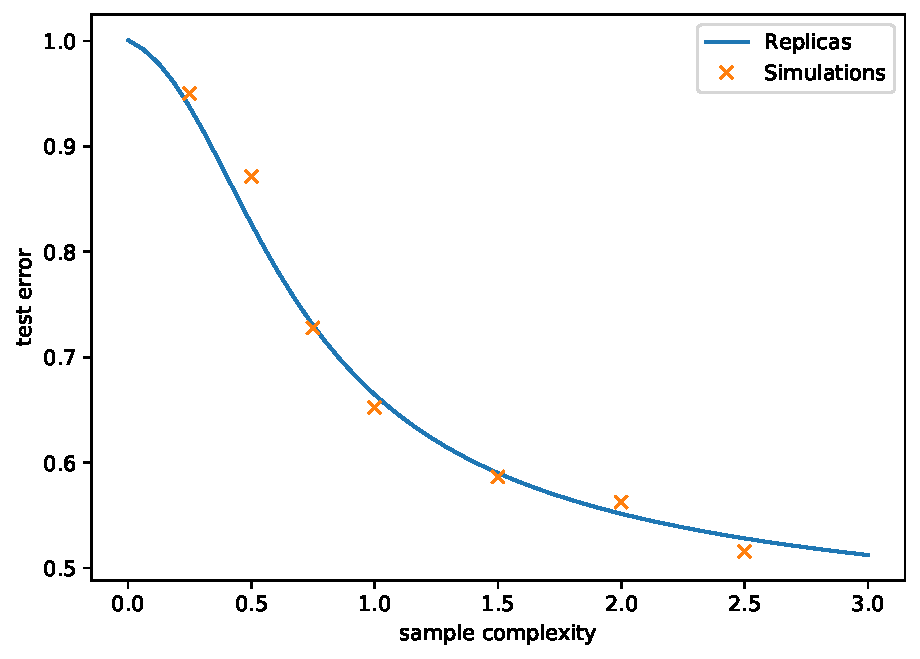
\includegraphics[scale=0.45]{../code/figs/check_ridge}
		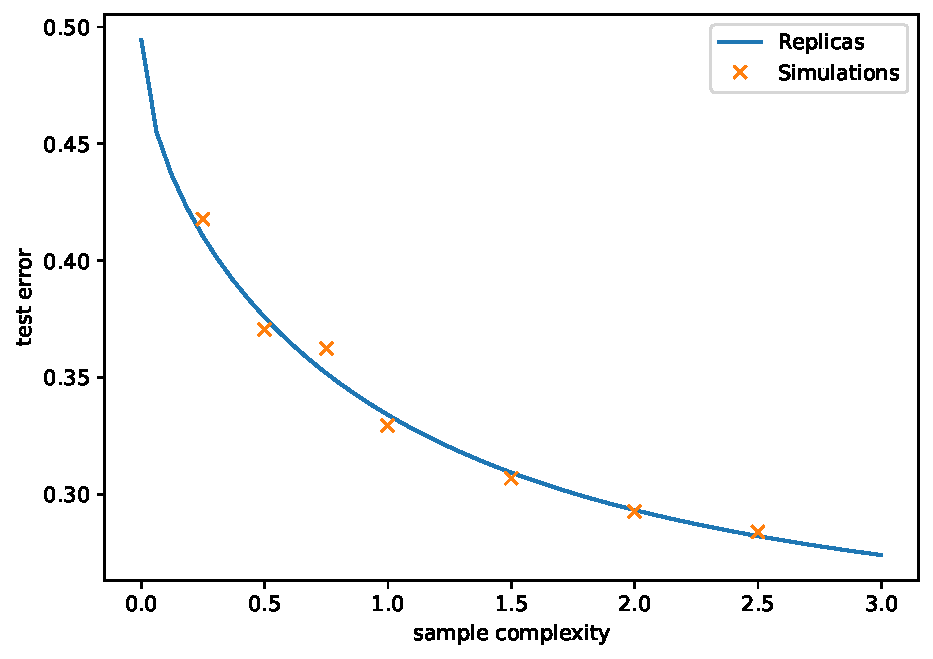
\includegraphics[scale=0.45]{../code/figs/check_logistic}
	\caption{Generalisation curves for the model defined in eq.~\eqref{eq:check1} for \textbf{(\textbf{left})} ridge regression and \textbf{(\textbf{right})} logistic regression, with $d/k = 1$, $d/p = 0.5$ and $\lambda = 0.01$.
	}
	\label{fig:check1}
\end{figure}



\end{document}


